\documentclass[11pt]{article}
\usepackage[utf8]{inputenc}
\usepackage[T1]{fontenc}
\usepackage{fixltx2e}
\usepackage{graphicx}
\usepackage{longtable}
\usepackage{float}
\usepackage{wrapfig}
\usepackage{rotating}
\usepackage[normalem]{ulem}
\usepackage{amsmath}
\usepackage{textcomp}
\usepackage{marvosym}
\usepackage{wasysym}
\usepackage{amssymb}
\usepackage[hidelinks]{hyperref}
\usepackage{listings}
\usepackage{xcolor}
\usepackage{amsthm}


\theoremstyle{definition}
\newtheorem{definition}{Definition}[section]

\lstdefinestyle{customc}{
  belowcaptionskip=1\baselineskip,
  breaklines=true,
  frame=L,
  numbers=left,
  stepnumber=1,
  tabsize=4,
  xleftmargin=\parindent,
  language=C,
  showstringspaces=false,
  basicstyle=\footnotesize\ttfamily,
  keywordstyle=\bfseries\color{green!40!black},
  commentstyle=\itshape\color{purple!40!black},
  identifierstyle=\color{blue},
  stringstyle=\color{orange},
}

\lstdefinestyle{customasm}{
  belowcaptionskip=1\baselineskip,
  frame=L,
  xleftmargin=\parindent,
  language=[x86masm]Assembler,
  basicstyle=\footnotesize\ttfamily,
  commentstyle=\itshape\color{purple!40!black},
}

\lstset{escapechar=@,style=customc}


\author{Sizhe Yuen}
\title{CS4052 Logic and Software Verification}

\begin{document}

\maketitle
\tableofcontents

\newcommand{\n}[0]{\\[\baselineskip]}

\section{Promela}

\subsection{Processes}
\begin{lstlisting}[caption={Process definition}]
proctype P1(int id) {
	int n = id;
	do 
	:: n < N -> n = n + 1;
	:: else -> break;
	od
}

active [N] proctype Pi() {
	//process is active on start and there are N processes
}

init {
	run P1(0);
}
\end{lstlisting}
More than one alternative can be given in a loop denoted by \texttt{::}. If more than one alternative is possible, choice is non-deterministic. 

\subsection{Channels}
\begin{lstlisting}[caption={Channel definition}]
chan toP1 = [0] of {byte}; //synchronous channel
chan toP2 = [N] of {byte}; //asynchronous channel with buffer size N

toP1!x; //send value of x down channel toP1
toP1?x; //receive message from channel toP1 into variable x
\end{lstlisting}
Synchronous channels block until the message is read while asynchronous channels block only when the buffer is full. 
\n
There are a number of functions that can be applied to a channel:
\begin{itemize}
\item \texttt{len(c)} - Number of messages in \texttt{c}
\item \texttt{empty(c)} - Is the channel empty?
\item \texttt{nempty(c)} - Is the channel not empty?
\item \texttt{full(c)} - Is the channel full?
\item \texttt{nfull(c)} - Is the channel not full?
\end{itemize}
There are also a number of variations of possible received messages:
\begin{itemize}
\item \texttt{c?x,y} - Received values saved to \texttt{x} and \texttt{y}
\item \texttt{c?2,y} - First sent value has to be 2
\item \texttt{c?eval(x),y} - First sent value must have the value of x
\item \texttt{c?<x,y>} - Received values saved to x and y, but message is kept in buffer
\item \texttt{c??2,y} - Get the first message in the buffer which has a first value of 2 (if none, keep waiting)
\item \texttt{c??<2,y>} - As above, but keep in buffer rather than read to variable y
\end{itemize}
Additional checks for asynchronous channels:
\begin{itemize}
\item \texttt{c?[x,y]} - Checks whether the message receipt is possible
\item \texttt{c?[2,y]} - Is \texttt{c?2,y} possible next?
\item \texttt{c??[2,y]} - Is \texttt{c??2,y} possible?
\end{itemize}
Note that we can also write \texttt{c?\_} if we do not care about the value being sent.

\subsection{Invariant}
An invariant is an example of a verifiable safety property which has to be true in all system states. In spin, assertions can be used as follows:
\begin{lstlisting}[caption={PROMELA assertion}]
assert(<Boolean condition>)

active proctype Invariant() {
	byte y = 0;
	bool b = false;
	assert( !b || y > 42);
}
\end{lstlisting}
Note the assertion above is only executed once. Labels can be used to block until a process reaches that label. For example:
\begin{lstlisting}[caption={PROMELA labels}]
active [3] proctype P() {
m1: do
	:: x < 10 -> m2: x = x + 1;
	:: x > 5 -> m3: break;
	od
}

active proctype Inv() {
	P[0]@m2;
	P[1]@m3;
	P[2]@m3;
	assert(x <= 11)
}
\end{lstlisting}

\subsection{Trace}
It is possible to impose specific sequences of communication using a \textbf{trace}.
\begin{lstlisting}[caption={Example of a trace}]
mtype = {a,b};
trace {
	do
	:: c1!a; c2?b;
	od
}
\end{lstlisting}
This above example states that \textit{sendong on channel \texttt{c1} alternates with receiving on channel \texttt{c2}}.
\section{LTL}

\subsection{Linear Time Properties}

\subsubsection{Safety}
Safety properties are about \textit{nothing bad should happen}. An example of this is the \textbf{mutual exclusion property} - Always at most one process is in its critical section.
\n
Safety properties refer to all states in the system.

\subsubsection{Liveness}
Liveness properties are about something good will happen eventually. They can be used to guarantee that progress is made.
\begin{itemize}
\item \textbf{Eventually} - Each process will eventually enter its critical section
\item \textbf{Repeated eventually} - Each process will enter its critical section infinitely often
\item \textbf{Starvation freedom} - Each waiting process will eventually enter its critical section
\end{itemize}
Liveness properties need to be checked for all possible system executions.

\subsubsection{Fairness}
\subsubsection*{Unconditional fairness}
Every process gets its turn infinitely often.

\subsubsection*{Strong fairness}
Every process that is \textbf{enabled} infinitely often gets its turn infinitely often.

\subsubsection*{Weak fairness}
Every process that is continuously enabled from a certain point onwards gets its turn infinitely often.

\begin{figure}[H]
\centering
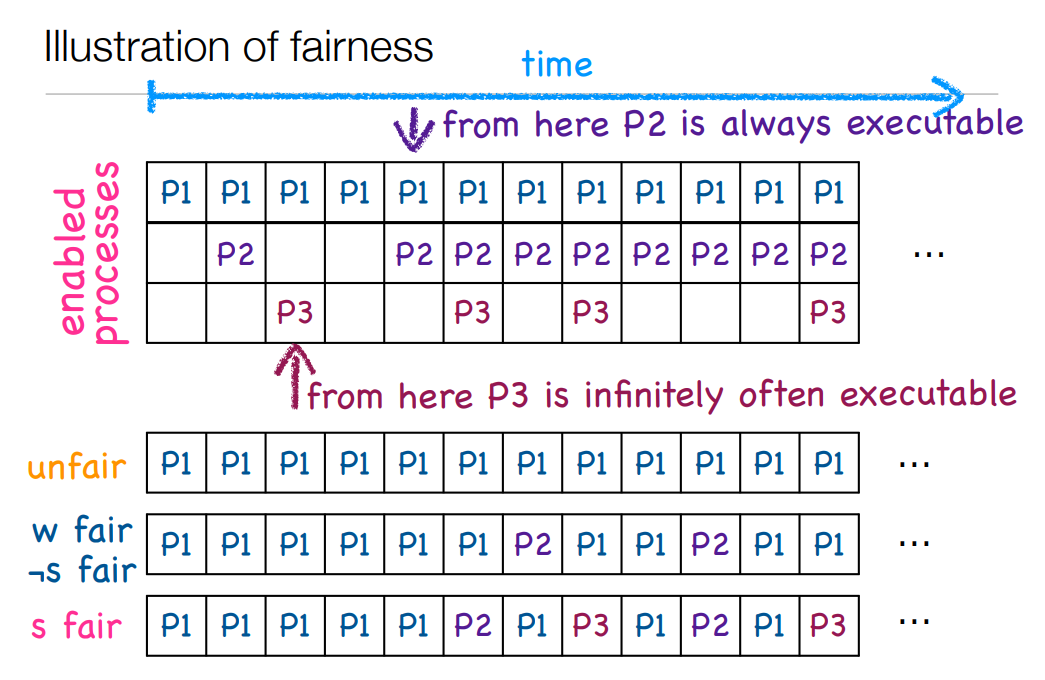
\includegraphics[width=1\textwidth, keepaspectratio]{imgs/fairness-example.png}
\caption{Illustration of fairness}
\end{figure}
\noindent
Spin supports weak fairness and can support strong fairness with an LTL statement.

\subsection{LTL}

\subsubsection{Syntax}
Given valid formulae $p$, $q$ and $r$:
\begin{itemize}
\item $\Box p$ - Always $p$
\item $\Diamond p$ - Eventually $p$
\item $\Circle p$ - Next $p$
\item $p\ U\ q$  - $p$ until $q$
\end{itemize}
There is a difference between strong and weak until. 

\begin{figure}[H]
\centering
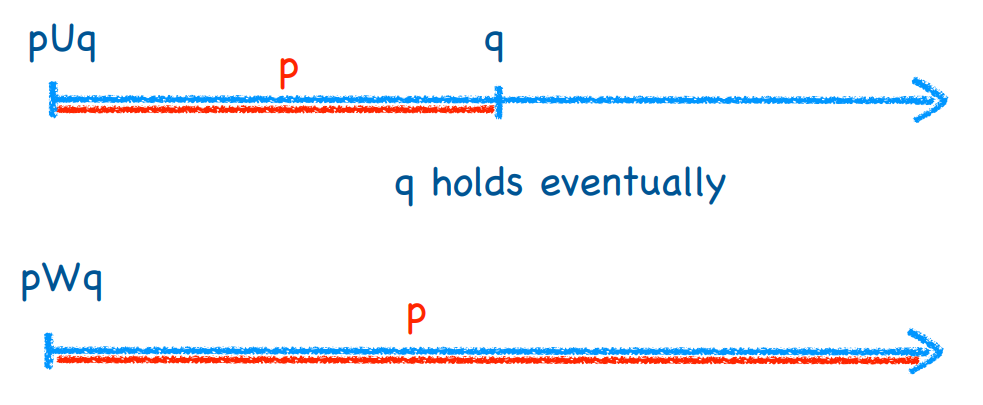
\includegraphics[width=0.9\textwidth, keepaspectratio]{imgs/strong-weak-until.png}
\caption{Strong and weak until}
\end{figure}

\subsubsection{Typical LTL Properties}
\begin{itemize}
\item{\makebox[5cm]{\textbf{Invariant}\hfill} $\Box p$}
\item{\makebox[5cm]{\textbf{Reply}\hfill} $p \rightarrow \Diamond q$}
\item{\makebox[5cm]{\textbf{Guaranteed reply}\hfill} $\Box (p \rightarrow \Diamond q)$}
\item{\makebox[5cm]{\textbf{Progress}\hfill} $\Box \Diamond p$ Infinitely often $p$}
\item{\makebox[5cm]{\textbf{Stability}\hfill} $\Diamond \Box p$ Eventually forever $p$}
\item{\makebox[5cm]{\textbf{Exclusion}\hfill} $\Box (p \rightarrow \neq q)$}
\end{itemize}

\subsubsection{LTL Properties for mutual exclusion}
\begin{itemize}
\item $P_{1}$ and $P_{2}$ never simultaneously have access to their critical sections:
\begin{equation}
\Box (\neg \text{crit}_{1} \vee \neg \text{crit}_{2})
\end{equation}

\item Each process is infinitely often in its critical section:
\begin{equation}
(\Box \Diamond \text{crit}_{1}) \wedge (\Box \Diamond \text{crit}_{2})
\end{equation}

\item Every waiting process will eventually enter its critical section:
\begin{equation}
(\Box \Diamond \text{wait}_{1} \rightarrow \Box \Diamond \text{crit}_{1}) \wedge (\Box \Diamond \text{wait}_{2} \rightarrow \Box \Diamond \text{crit}_{2})
\end{equation}

\item Whenever the semaphore $y$ has the value 0, one of the processes is in its critical section:
\begin{equation}
\Box (y = 0 \rightarrow \text{crit}_{1} \vee \text{crit}_{2})
\end{equation}
\end{itemize}

\subsubsection{Fairness in LTL}
Three types of fairness constraints:
\begin{itemize}
\item{\makebox[3cm]{Unconditional\hfill}} $\Box \Diamond \text{crit}_{i}$
\item{\makebox[3cm]{Strong fairness\hfill}} $\Box \Diamond \text{wait}_{i} \rightarrow \Box \Diamond \text{crit}_{i}$
\item{\makebox[3cm]{Weak fairness\hfill}} $\Diamond \Box \text{wait}_{i} \rightarrow \Box \Diamond \text{crit}_{i}$
\end{itemize}


\subsection{Transition System}
\begin{equation}
TS = (S, Act, T, I, AP, L)
\end{equation}
where
\begin{align*}
\makebox[3cm]{S\hfill} &= \text{set of states} \\
\makebox[3cm]{Act\hfill} &= \text{set of actions} \\
\makebox[3cm]{T\subseteq S \times Act \times S\hfill} &= \text{transition relation} \\
\makebox[3cm]{I\subseteq S\hfill} &= \text{set of initial states} \\
\makebox[3cm]{AP\hfill} &= \text{set of atomic propositions} \\
\makebox[3cm]{L:S \rightarrow 2\textsuperscript{AP}\hfill} &= \text{labelling function} 
\end{align*}

\subsubsection{Deterministic observable behaviour}
\textbf{Action based}: deterministic on the executed observable actions. \textit{At most one outgoing transition labelled with action \alpha per state}
\n
\textbf{State based}: ignore actions and reply on APs that hold in the current state. \textit{At most one outgoing transition from a state with label \texttt{a} to a state with label \texttt{a}}

\subsubsection{Execution fragment}
Let $TS = (S, Act, T, I, AP, L)$ \\
A finite execution of fragment \rho\ of TS is an alternating sequence of states and actions ending with a state:
\begin{equation}
\rho = s_{0}\ \alpha_{1}\ s_{1}\ \alpha_{2}\ s_{2}\ ...\ \alpha_{n}\ s_{n}
\end{equation}
such that $(s_{i}, \alpha_{i+1}, s_{i+1}) \in T\ \text{forall}\ 0 \leq i < n\ \text{where}\ n \geq 0$.
\\
\begin{itemize}
\item An \textbf{execution fragment} \rho\ of TS can also be infinite.
\item A \textbf{maximal execution fragment} is either finite ending in a terminal state, or infinite.
\item An \textbf{initial execution fragment} starts in an initial state.
\end{itemize}
A state $s \in\ S$ is \textbf{reachable} in TS if there exists an initial, finite execution fragment:
\begin{equation*}
\rho = s_{0}\ \alpha_{1}\ s_{1}\ \alpha_{2}\ s_{2}\ ...\ \alpha_{n}\ s_{n} = s
\end{equation*}
with $s_{0} \in I$ and $n \geq 0$

\subsection{Program Graphs}
A program graph over a set \texttt{Var} of typed variables is defined as follows:
\begin{equation}
PG = (Loc, Act, \text{Effect}, C_{\dagger}, Loc_{0}, g_{0})
\end{equation}
where
\begin{align*}
\makebox[7cm]{Loc\hfill} &= \text{set of locations} \\
\makebox[7cm]{Act\hfill} &= \text{set of actions} \\
\makebox[7cm]{Effect: $Act \times Eval(var) \rightarrow\ Eval(var)$\hfill} &= \text{effect function} \\
\makebox[7cm]{$C_{\dagger} \subseteq Loc \times Cond(var) \times Act \times Loc$\hfill} &= \text{conditional transition relation} \\
\makebox[7cm]{$Loc_{0} \subseteq Loc$\hfill} &= \text{set of initial locations} \\
\makebox[7cm]{$g_{0}\in Cond(Var$\hfill} &= \text{initial condition}
\end{align*}
\noindent
The \textbf{Effect} indicates how the evaluation $\eta$ of variables is changed by performing an action.

\subsubsection{Transition System for a Program Graph}
The $TS(PG)$ of a $PG=(Loc, Act, \text{Effect}, C_{\dagger}, Loc_{0}, g_{0})$ over Var is the following tuple:
\begin{equation}
TS(PG) = (S, Act, T, I, AP, L)
\end{equation}
where
\begin{align*}
\makebox[3cm]{S\hfill} &= Loc \times Eval(Var) \\ \\
\makebox[3cm]{T\subseteq S \times Act \times S\hfill} &= \frac{l_{1} \xrightarrow[]{g:\alpha} l_{2} \wedge \eta \vDash g}{\langle l_{1}, \eta \rangle \xrightarrow[]{\alpha} \langle l_{2}, \text{Effect}(\alpha, \eta) \rangle} \\ \\
\makebox[3cm]{I\hfill} &= \{\langle l,\eta \rangle\ |\ l \in Loc_{0} \wedge \eta \vDash g_{0} \} \\ \\
\makebox[3cm]{AP\hfill} &= Loc \cup Cond(Var) \\ \\
\makebox[3cm]{$L(\langle l, \eta \rangle) $\hfill} &= \{ l \} \cup \{ g \in Cond(Var)\ |\ \eta \vDash g\}
\end{align*}

\subsection{Parallel Composition of Transition Systems}
\begin{equation}
TS = TS_{1}\ \|\ TS_{2}\ \|\ ...\ \|\ TS_{n}
\end{equation}
$\|$ is the parallel composition operator and is usually \textbf{commutative} and \textbf{associative} but depends on the kind of communication supported.
\n
$|||$ is the \textbf{interleaving} operator where the actions from different processes are interleaved and the system is made of a set of independent processes (no communication).
\n
The interleaving operator for transition systems simply constructs the \textbf{Cartesian product} of the individual state spaces without considering the potential conflicts from \textit{shared} variables. For programs with shared variables, we define interleaving directly on the program graph level: $PG_{1}\ |||\ PG_{2}$.

\subsubsection{Composed Program Graph $PG_{1}\ |||\ PG_{2}$}
\begin{itemize}
\item Local variables of $PG_{1}$ are $x_{1} \in Var_{1} \setminus Var_{2}$
\item Local variables of $PG_{2}$ are $x_{2} \in Var_{2} \setminus Var_{1}$
\item \textbf{Global} variables are $x \in Var_{1} \cap Var_{2}$
\end{itemize}
Actions that access global variables are \textbf{critical} and critical actions \textit{cannot be executed simultaneously}.


\subsubsection{Handshaking $TS_{1} \|_{H} TS_{2}$}
Handshaking allows for processes to interact at the same time through synchronous communication (shared actions). The composition of two transition systems handshaking on actions $H$ is as follows:
\begin{equation}
TS_{1} \|_{H} TS_{2} = (S_{1} \times S_{2}, Act_{1} \cup Act_{2}, T, I_{1} \times I_{2}, AP_{1} \cup AP_{2}, L)
\end{equation}
where $H \subseteq Act_{1} \cap Act_{2}$.
\n
Transitions for synchronisation means the actions in $H$ are taken \textit{synchronously} by both processes:
\begin{equation}
\frac{(s_{1} \xrightarrow[]{\alpha}_{1} s'_{1}) \wedge (s_{2} \xrightarrow[]{\alpha}_{2} s'_{2})}{\langle s_{1}, s_{2} \rangle \xrightarrow[]{\alpha} \langle s'_{1}, s'_{2} \rangle}
\end{equation}
Note that if there is no synchronisation of actions, it is the same as interleaving:
\begin{equation}
TS_{1}\ \|_{\emptyset}\ TS_{2} = TS_{1}\ |||\ TS_{2}
\end{equation}


\section{Timed Automata}
Timed automata add clock variables to the program graph. A clock constraint over a set of $C$ of clocks is formed as follows:
\begin{equation}
g ::= x < c | x \leq c | x > c | x \geq c | g \wedge g
\end{equation}
where $c$ is a natural number and $x \in C$.
\subsection{Definition}
A Timed Automata is the tuple $TA = (Loc, Act, C, C_{t}, Loc_{0}, Inv, AP, L$ where:
\begin{align*}
C &= \text{Finite set of clock} \\
Inv &= Loc \rightarrow CC(C)
\end{align*}

\subsection{Handshaking with timed automata}
\textbf{Synchronisation}
\begin{equation}
\frac{l_{1} \xrightarrow[]{g_{1}:\alpha, D_{1}}_{1} l'_{1} \wedge l_{2} \xrightarrow[]{g_{2}:\alpha, D_{2}}_{2} l'_{2}}{\langle l_{1}, l_{2} \rangle \xrightarrow[]{g_{1} \wedge g_{2}:\alpha, D_{1} \cup D_{2}} \langle l'_{1}, l'_{2} \rangle}
\end{equation}

\textbf{Interleaving}
\begin{equation}
\frac{l_{1} \xrightarrow[]{g:\alpha, D}_{1} l'_{1}}{\langle l_{1}, l_{2} \rangle \xrightarrow[]{g:\alpha, D} \langle l'_{1}, l_{2} \rangle}\ \text{or}\ \frac{l_{2} \xrightarrow[]{g:\alpha, D}_{2} l'_{2}}{\langle l_{1}, l_{2} \rangle \xrightarrow[]{g:\alpha, D} \langle l_{1}, l'_{2} \rangle}
\end{equation}

\subsection{CTL Syntax}
State formula of a set of AP are formed according to the following grammar:
\begin{equation}
\Phi ::= true\ |\ a\ |\ \Phi \wedge \Phi\ |\ \neg \Phi\ |\ \exists \phi\ |\ \forall \phi
\end{equation}
where $\phi$ is a path formula:
\begin{equation}
\phi ::= \Circle \Phi\ |\ \Phi \cup \Phi
\end{equation}

\subsubsection{CTL properties}
\begin{itemize}
\item There exists an execution along which $p$ will eventually hold:
\begin{equation}
\exists \Diamond p
\end{equation}
\item There exists an execution along which $p$ is always true:
\begin{equation}
\exists \Box p
\end{equation}
\item Necessarily $p$ will eventually hold
\begin{equation}
\forall \Diamond p
\end{equation}
\item $p$ is always true
\begin{equation}
\forall \Box p
\end{equation}
\end{itemize}

\subsubsection{CTL examples}
\begin{itemize}
\item $P_{1}$ and $P_{2}$ are never simultaneously in their critical sections:
\begin{equation}
\forall \Box (\neg \text{crit}_{1} \vee \neg \text{crit}_{2})
\end{equation}

\item Each process is infinitely often in its critical section:
\begin{equation}
(\forall \Box \forall \Diamond \text{crit}_{1}) \wedge (\forall \Box \forall \Diamond \text{crit}_{2})
\end{equation}
\end{itemize}

\subsubsection{Derivations for eventually and always}
\textbf{Eventually}
\begin{align*}
\exists \Diamond \Phi &= \exists (true \cup \Phi) \\
\forall \Diamond \Phi &= \forall (true \cup \Phi)
\end{align*}
\textbf{Always}
\begin{align*}
\exists \Box \Phi &= \neg \forall \Diamond \neg \Phi \\
\forall \Box \Phi &= \neg \exists \Diamond \neg \Phi 
\end{align*}

\subsection{Timed CTL (TCTL)}
\textbf{Eventually}
\begin{align*}
\exists \Diamond^{J} \Phi &= \exists(true \cup^{J} \Phi) \\
\forall \Diamond^{J} \Phi &= \forall(true \cup^{J} \Phi)
\end{align*}
\textbf{Always}
\begin{align*}
\exists \Box^{J} \Phi &= \neg \forall \Diamond^{J} \neg \Phi \\
\forall \Box^{J} \Phi &= \neg \exists \Diamond^{J} \neg \Phi 
\end{align*}
$J$ denotes the time interval, for example:
\begin{align*}
\Diamond^{\leq 2}\ &\text{denotes}\ \Diamond^{[0,2]} \\
\Diamond^{>8}\ &\text{denotes}\ \Diamond^{[8,\infty[} \\
\Diamond\ &\text{denotes}\ \Diamond^{[0,\infty[}
\end{align*}
\subsubsection{Definition}
There exists a path in which $\Phi$ holds during interval $J$:
\begin{equation}
\exists \Box^{J} \Phi
\end{equation}
In all paths $\Phi$ must hold during interval $J$:
\begin{equation}
\forall \Box^{J} \Phi
\end{equation}

\subsubsection{Example TCTL Properties}
The light cannot be continuously on for more than 2 time units:
\begin{equation}
\forall \Box (on \rightarrow \forall \Diamond^{\leq 2} \neg on)
\end{equation}
The light will stay on for at least 1 time unit and then switch off:
\begin{equation}
\forall \Box (on \rightarrow (\forall \Box^{\leq 1} on \wedge \forall \Diamond^{>1} \text{off}))
\end{equation}
The gate is always closed when the train is at the crossing:
\begin{equation}
\forall \Box (crossing \rightarrow closed)
\end{equation}
Once the train is far, within one minute the gate is up for at least 1 minute:
\begin{equation}
\forall \Box (\text{far} \rightarrow \forall \Diamond^{\leq 1} \forall \Box^{\leq 1} up)
\end{equation}

\subsection{UPPAAL}

\section{Petri Nets}

\subsection{Definition}
A Petri net is a tuple $N = (P, T, G)$ where:
\begin{itemize}
\item $P$ is a set of \textbf{places}
\item $T$ is a set of \textbf{transitions}
\item $G$ is a directed graph linking places and transitions
\end{itemize}

\subsection{Reachability}
Let $M$ ba a marking for a Petri net $N = (P, T, G)$:
\begin{equation}
\text{Reachable}(N,M) = \{M'\ |\ M'\ \text{is a marking for}\ N\}
\end{equation}
such that there is a sequence of enabled transitions $t_{i} \in T$ with $0 \leq i \leq n$ which leads to $M'$
\n
The set can be finite and infinite and a marking for which there is no enabled transition indicates a deadlock. 

\end{document}

